\documentclass[10pt,a4paper]{article}
\usepackage[utf8]{inputenc}
\usepackage{amsmath}
\usepackage{amsfonts}
\usepackage{amssymb}
\usepackage[spanish]{babel}

\usepackage{pdflscape}
\usepackage{afterpage}

\usepackage{float}
\usepackage[table,xcdraw]{xcolor} %para usar tablas con color de fondo en las celdas
\usepackage{hyperref} %para poder poner enlaces
\usepackage{listings} %para insertar código
\usepackage{tikz}%para pintar las redes neuronales
%\usepackage{color} %para poder definir y usar colores
\usepackage{soulutf8} %para hacer los subrayados

\usepackage{sectsty} %cambiar el color del título de las secciones y subsecciones


\author{\textbf{Gustavo Rivas Gervilla}}
\title{\textcolor{deepblue}{\textbf{Titanic. Competición Kaggle.}}}
\date{}

%Configurando lstlisting para mostrar código Python con algún 	 de colores (copiado de http://tex.stackexchange.com/questions/83882/how-to-highlight-python-syntax-in-latex-listings-lstinputlistings-command) ------------------------------
% Custom colors
\definecolor{deepblue}{RGB}{12, 17, 104}
\definecolor{rblue}{rgb}{0.2,0.6,1}
\definecolor{deepgreen}{rgb}{0,0.5,0}
\definecolor{light-gray}{gray}{0.85}
\definecolor{comment-gray}{gray}{0.65}
\definecolor{light-blue}{rgb}{0.6,1,0.8}
\definecolor{light-yellow}{rgb}{1,1,0.6}

% Default fixed font does not support bold face
\DeclareFixedFont{\ttb}{T1}{txtt}{bx}{n}{8} % for bold
\DeclareFixedFont{\ttm}{T1}{txtt}{m}{n}{8}  % for normal

%Configuración de los listings
\lstset{
	language=Python,
	basicstyle=\ttm,
	otherkeywords={self},             % Add keywords here
	keywordstyle=\ttb\color{deepblue},
	emph={MyClass,__init__},          % Custom highlighting
	emphstyle=\ttb\color{deepred},    % Custom highlighting style
	stringstyle=\color{deepgreen},
	frame=tb,                         % Any extra options here
	showstringspaces=false,            % 
	commentstyle=\ttm\color{comment-gray}, % Custom comment style
}
%--------------------------------------------------------------------------------

\newcommand{\emp}[1]{\sethlcolor{light-yellow}\hl{#1}} %Comando para poner código inline
\newcommand{\code}[1]{\textcolor{rblue}{\texttt{#1}}} %Comando para poner código inline
\newcommand{\archive}[1]{\sethlcolor{light-blue}\hl{\texttt{#1}}} %Comando para resaltar nombres de archivos
\renewcommand\tablename{Tabla} %Cambiar el nombre de las tablas
\renewcommand\figurename{Figura} %Cambiar el nombre de las tablas
\renewcommand{\contentsname}{Índice} %Cambiar el nombre de la ToC

\usepackage{pdfpages}

\hypersetup{
    colorlinks,
    linkcolor={red!50!black},
    citecolor={blue!50!black},
    urlcolor={blue!80!black}
}

\sectionfont{\color{deepblue}}
\subsectionfont{\color{blue}}

\begin{document}
\maketitle

\begin{center}
  \textbf{Nombre del equipo: }Gustavo Rivas Gervilla\\
  \textbf{Ranking global: }417\\
  \textbf{Puntuación: }0.81340
\end{center}

\newpage

\tableofcontents

\newpage

\section{Introducción}

En este trabajo se va a trabajar con el dataset del Titanic, un conjunto de datos en el que se plantea un \textbf{problema de clasificación}, dadas una serie de características de un pasajero, que enumeraremos en la siguiente sección, se tendrá que decidir si el pasajero sobrevivió o no a la catastrofe. En primer lugar, como toma de contacto con el dataset y también para tomar algunas ideas que aplicar al conjunto de datos, se han realizado dos tutoriales con planteamientos similares, ambos realizan un preprocesamiento parecido a los datos y emplean Random Forest como algoritmo final de clasificación, después de probar otros modelos como puede ser uno basado en un árbol de decisión o simplemente suponer que todas las mujeres sobrevivieron y que todos los hombres perecieron. La realización de estos dos tutoriales se adjunta en esta memoria a modo de apéndices.\\

\section{Exploración de datos} \emph{Ver archivo \archive{exploracion.Rmd}}\\

En primer lugar vamos a presentar el conjunto de datos que tenemos, disponemos de 891 instancias en el conjunto de entrenamiento y 418 en el conjunto de test. Estas instancias presentan el siguiente conjunto de atributos:

\begin{enumerate}
\item \textbf{PassengerId: } identificador del pasajero.
\item \textbf{Pclass: } la clase en la que embarcó.
\item \textbf{Name:} el nombre del pasajero.
\item \textbf{Sex: } sexo del pasajero.
\item \textbf{Age: } edad del pasajero.
\item \textbf{SibSp: } número de hermanos/esposos/esposas del pasajero que viajaban también a bordo.
\item \textbf{Parch: } número de padres/hijos del pasajero que viajaban también a bordo.
\item \textbf{Ticket: } número o identificador del ticket de embarque del pasajero.
\item \textbf{Fare: } lo que pagó el pasajero por su pasaje.
\item \textbf{Cabin: } camarote(s) en el(los) que viajó el pasajero.
\item \textbf{Embarked: } puerto desde el que embarcó. C = Cherbourg, Q = Queenstown, S = Southampton.
\item \textbf{Survived: } el pasajero murió (0) o sobrevivió (1). La variable a predecir y que por tanto no está presente en las intancias del conjunto de test.
\end{enumerate}

Lo primero que hemos hecho ha sido estudiar si contábamos con valores perdidos. Gracias a los tutoriales notamos que hay algunos atributos que, si bien no presentan valores perdido (\textbf{NA}), contienen una cadena vacía, lo que se podría considerar también un valor perdido, y por lo tanto esto también se tendrá en cuenta en la fase de preprocesamiento. Tras este análisis vemos que la mayoría de valores perdidos están en el atributo \textbf{Age}, también hay algún valor perdido en el \textbf{Embarked} y muchos valores perdidos para el atributo \textbf{Cabin} (señalar aquí que en R es mejor emplear los operandos condiciones \code{\&} y \code{|}, en lugar de \texttt{\&\&} o \texttt{||}, ya que con estos obtenemos resultados incorrectos). Para estudiar de forma general el conjunto de datos de los que disponemos han sido de utilidad los métodos \code{summary} y \code{str}.\\

De hecho en ambos conjuntos, para el atributo \textbf{Cabin} tenemos aproximadamente un 78\% de valores perdidos, lo cual es una cantidad muy elevada. En el tutorial sobre ingeniería de características que se facilita desde la propia página de la competición se habla de obtener, procesando este campo, la cubierta en la que se alojó el pasajero. Sin embargo, puesto que se trata de un atributo con tantos valores perdidos se ha decidido no realizar dicho preprocesamiento: no tenemos información suficiente para decidir en qué cubierta viajó el pasajero y una imputación, usando por ejemplo el paquete \code{mice}, no sería de mucha confianza al tener un número tan elevado de valores perdidos.\\

Vamos a ver ahora la primera gráfica sobre nuestro conjunto de datos, lo que vamos a reflejar en esta gráfica es el desequilibrio entre las dos clases (549 muertos y 342 sobrevivientes), aunque no se trata de un desequilibrio demasiado grande lo trataremos en la fase de preprocesamiento y trataremos de comparar distintas técnicas de balanceo de clases según su rendimiento para un algoritmo determinado:

\begin{figure}[H]
  \centering
  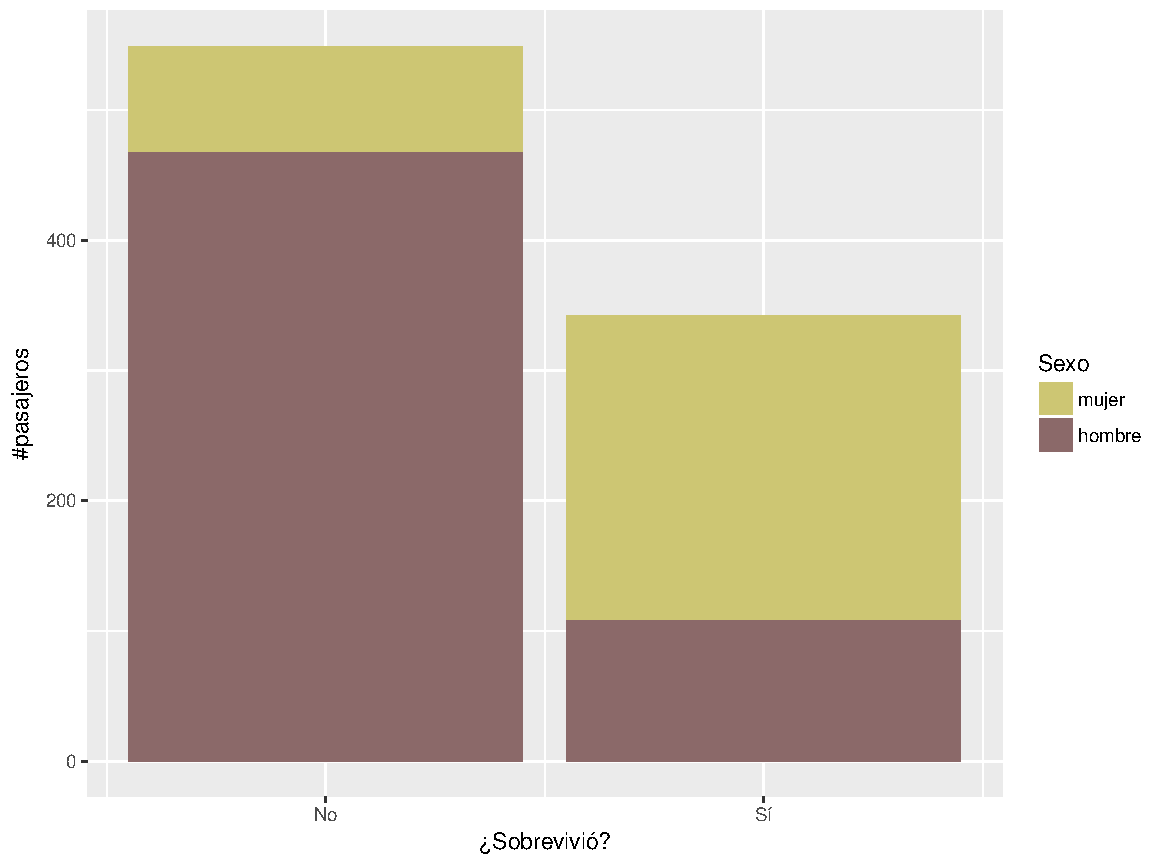
\includegraphics[width=\textwidth]{imgs/imbalanced.pdf}
  \caption{Desbalanceo entre clases}
\end{figure}

En la gráfica anterior también mostramos en qué proporción sobreviven hombres y mujeres en el conjunto de entrenamiento. Como podemos ver son las mujeres las que en su mayoría sobrevivieron mientras que los hombres tuvieron menos posibilidades, recordemos que durante el accidente del Titanic se estableció la política de evacuar a mujeres y niños en primer lugar. Este hecho nos lleva, en el tutorial de Trevor Stephens, a plantear el modelo sexista.

\begin{figure}[H]
  \centering
  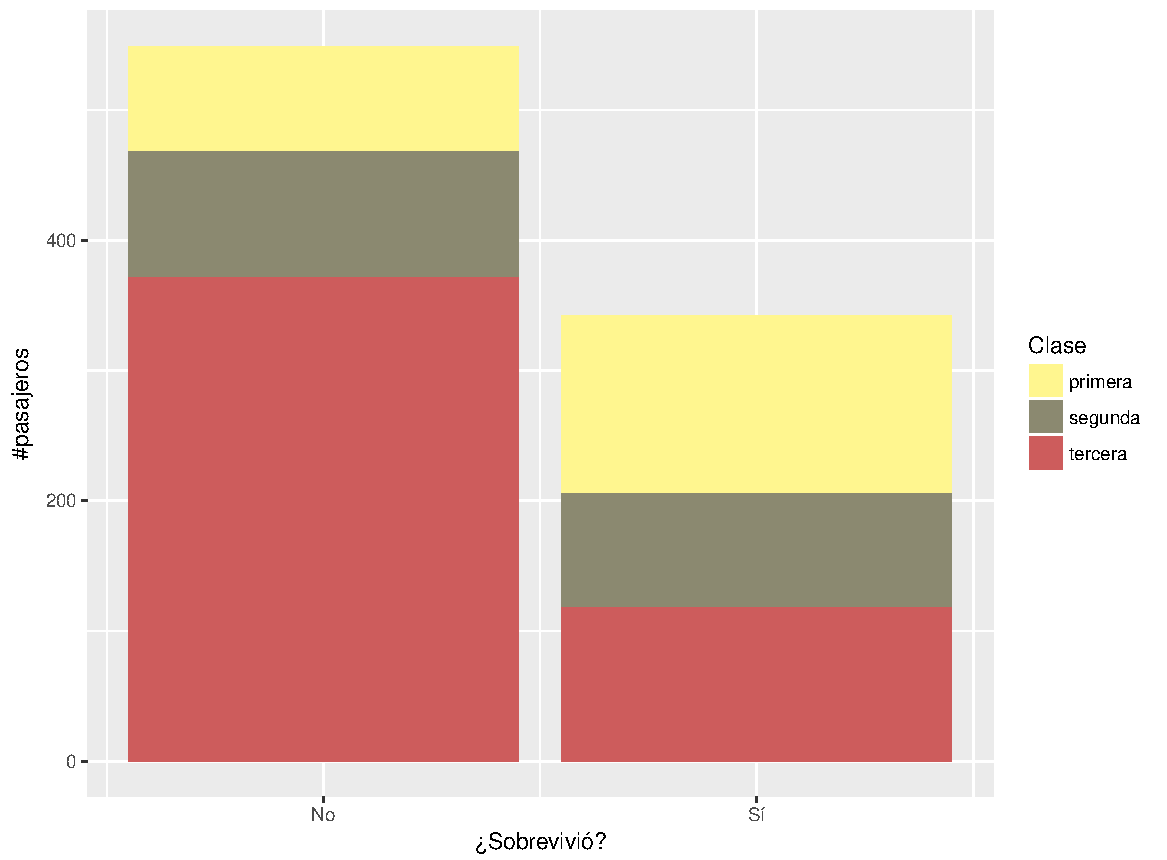
\includegraphics[width=\textwidth]{imgs/classes.pdf}
  \caption{Distribución de sobrevivientes según la clase}
\end{figure}

En esta gráfica lo que vemos es cómo se distribuyen los sobrevivientes en las distintas clases de los pasajeros. Como vemos son los de tercera clase los que perecieron en mayor proporción. Sin embargo observamos algo interesante, y es que en los sobrevivientes lo parece haber tanta diferencia entre las clases, siendo los pasajeros de segunda clase y no los de tercera los que murieron en mayor proporción. Como vemos el análisis exploratorio ha sido principalemente enfocado a ver cómo influyen las distintas características de los pasajeros en su probabilidad de sobrevivir, al fin y al cabo este es el problema que se nos plantea con este dataset.\\

\begin{figure}[H]
  \centering
  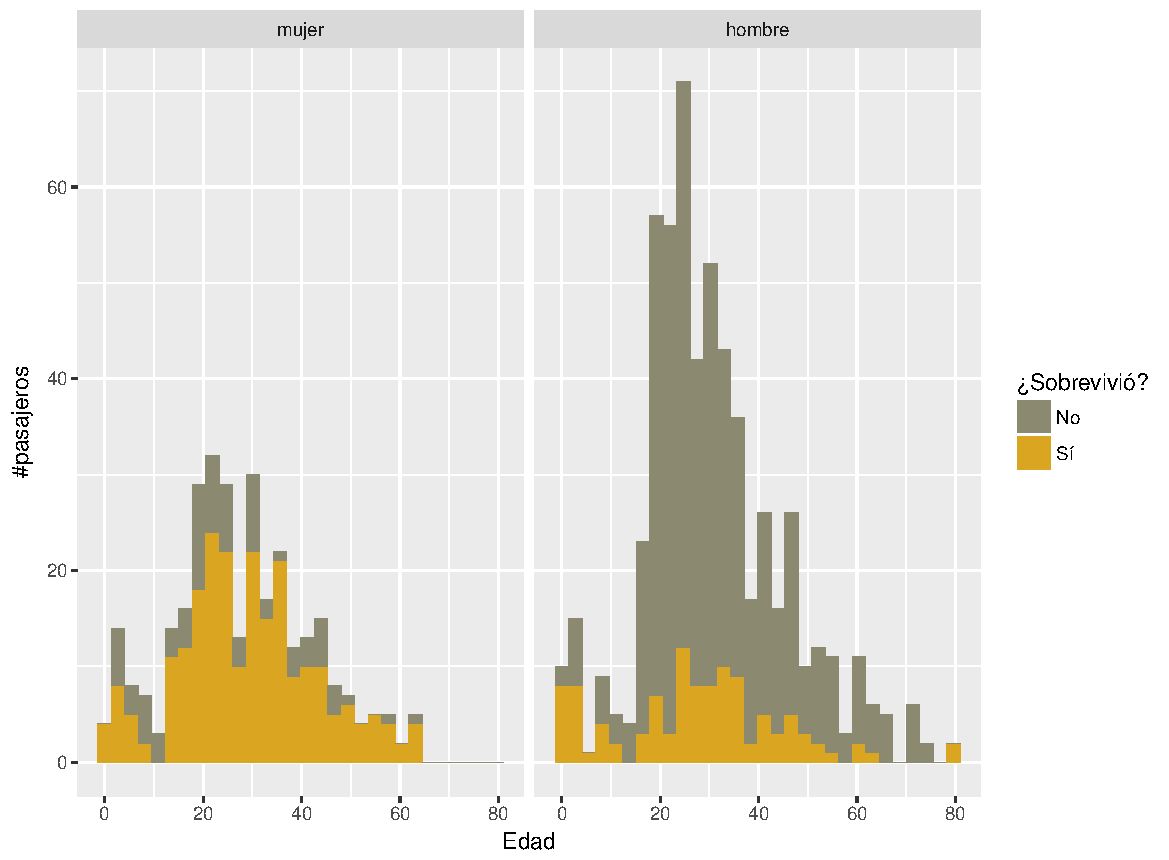
\includegraphics[width=\textwidth]{imgs/age.pdf}
  \caption{Distribución de sobrevivientes según la edad y el sexo.}
\end{figure}

Aquí lo que podemos apreciar es en primer lugar que las mujeres sobreviven en mayor proporción que los hombres, por otro lado los hombres jóvenes parecen sobrevivir en mayor proporción que los mayores, al contrario que ocurre con las mujeres.

\begin{figure}[H]
  \centering
  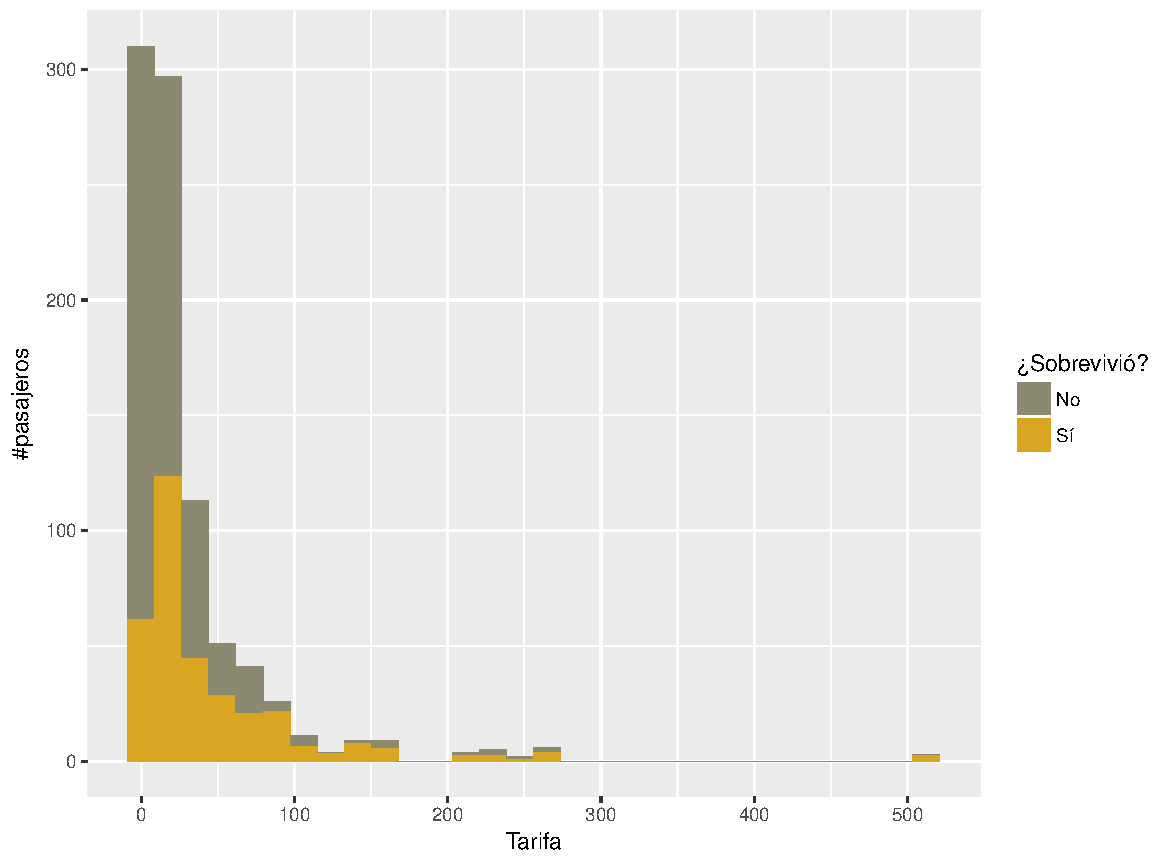
\includegraphics[width=\textwidth]{imgs/fare.pdf}
  \caption{Distribución de sobrevivientes según la edad y el sexo.}
\end{figure}

En esta gráfica apreciamos algo parecido a lo que teníamos en la gráfica con las clases de los pasajeros. Los pasajeros que pagaron menos por su pasaje, los de menor clase suponemos, son los que mueren en mayor proporción. Claro hay muerte que no se corresponden con esto, pensemos en que aquí estamos analizando los factores uno por uno por separado. Hay muchos factores distintos que pudieron influir en la muerte de un pasajero, entre otros su localización en el barco. Como ya hemos dicho este no es un factor que nosotros hayamos tenido en cuenta, y queda como trabajo futuro.\\

Por último vamos a ver cómo se distribuye la tasa de muertos según el tamaño de la familia. Parece lógico pensar que se intentó evacuar a las familias juntas, o que estas presionaron para que se evacuasen a todos sus miembros. Sin embargo, familias con un tamaño muy grande es más complicado que se pudiesen evacuar y quizás, por tal de permanecer unidas perecieran. Por tanto esta variable que se crea nueva, el tamaño de la familia, puede resultar muy interesante:

\begin{figure}[H]
  \centering
  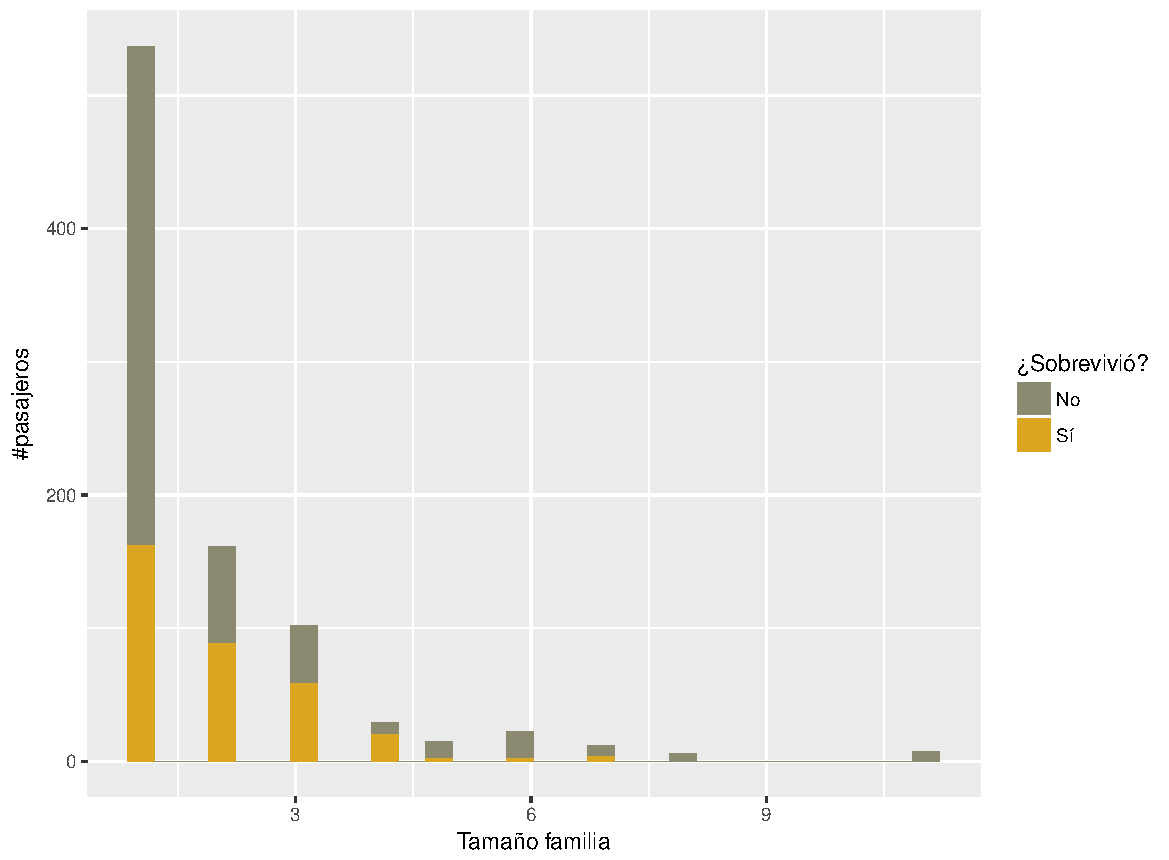
\includegraphics[width=\textwidth]{imgs/fsize.pdf}
  \caption{Distribución de sobrevivientes según el tamaño de su familia.}
\end{figure}

Como podemos ver aquellos pasajeros que viajaban solos tenían mayor probabilidad de morir y por otro lado, las familias con un tamaño demasiado grande, cinco miembros o más, también lo tenían más difícil para sobrevivir.

\section{Preprocesamiento} \emph{Ver archivo \archive{preprocesamiento.Rmd}}\\

Hemos dividido el preprocesamiento en 3 fases. La primera en la que tendríamos el preprocesamiento de los datos que tenemos originales, lo que sería la ingeniería de características y la imputación de valores perdidos. Luego pasamos a una fase de balanceo de clases donde se prueban 3 técnicas distintas de balanceo, y por último limpiamos ruido por medio del algoritmo IPF.

\subsection{Preprocesamiento básico}


Lo primero que hemos hecho ha sido \emp{fabricar una nueva variable que recoge el título de cada pasajero}, para ello hemos extraído este título del nombre de cada pasajero. El título podría darnos información de la clase social del pasajero y quizás aquellos pasajeros de mayor estatus tuvieron mayor posibilidad de ser evacuado. El \textit{problema} que presenta esta variable es que presenta muchos valores distintos a lo largo de los \textit{datasets} con lo cual lo que hemos hecho es agrupar distintos títulos es uno solo.\\

Muchos de estos títulos son equivalente, con lo cual tener una granularidad tan alta en una variable quizás lo único que haría sería provocar que nuestros modelos funcionasen peor al introducir una componente de sobreajuste en los mismo. Hemos probado distintos agrupamientos, se puede ver en el código uno de ellos comentado, sin embargo, y aunque las diferencias eran mínimas se ha optado por dejar el agrupamiento que hace Trevor Stephens, para obtener el mejor resultado. Pensemos que hablamos de un conjunto de test muy pequeño y pequeñas variaciones en las predicciones dan lugar a cambios en la tasa de acierto de uno o dos puntos, que son las diferencias con las que nos solemos mover.\\

A continuación lo que hemos hecho ha sido \emp{crear una variable que recoge el tamaño de la familia del pasajero a bordo} contándolo a él, y combinando ésta con el apellido de cada pasajero, se \emp{fabrica una nueva variable que se puede ver como un identificador para la familia abordo del pasajero}. Esta variable tiene sentido ya que, si bien pensamos que familias demasiado grandes pudieron tener más problemas para ser evacuadas, puede que unas familias, por su estatus, tuviesen más fácil el ser evacuadas. Combinamos las dos variables y no usamos únicamente el apellido para intentar no mezclar personas de distintas familias dentro del mismo identificador.\\

No obstante, para que esta variable no tenga una granularidad muy elevada (por ejemplo el Random Forest del paquete \code{randomForest} no admite variables de tipo factor con más de 32 niveles), hemos asignado todas las familias con 2 miembros o menos en un mismo identificador \code{'Small'}, esto concuerda con lo que vimos en la sección de exploración, aquellos que viajaban solos tenían más posibilidades de morir, aunque quizás sí que penaliza a las familias de dos miembros.\\

A continuación lo que hacemos es \emp{imputar los valores perdidos para el atributo \textbf{Embarked}}, esto sólo ocurre en dos instancias del conjunto de datos, y dado que las dos pasajeras no cuenta de familiares a bordo con los que poder deducir el puerto desde el que embarcaron, ambas pagaron lo mismo por su pasaje(80\$) en primera clase y Southhampton es el puerto más frecuente, además de que la media de la tarifa de embarque en primera clase desde este puerto es de aproximadamente 72\$, decidimos asignarle a ambas pasajeras dicho puerto. En el tutorial de Megan Risdal en cambio se le asigna el puerto \code{C} que tiene una media de precio de 90\$ y es menos frecuente que el \code{S}. Nosotros hemos optado por la idea que se da en el tutorial de Trevor Stephens. De todos modos estamos hablando de una decisión que sólo afecta a dos instancias del conjunto completo de datos con lo que no es algo crítico.\\

Algo más simple fue la decisión para \emp{imputar el único valor perdido que tenemos para el atributo \textbf{Fare}}, lo único que hemos hecho ha sido asignarle al pasajero del que no conocemos la tarifa que pagó la media de lo que pagaron otros pasajeros con sus mismas características (embarcaron desde el mismo puerto y en la misma clase que él).\\

Luego lo que hicimos fue \emp{imputar los valores perdidos para el atributo \textbf{Age}}, para este atributo sí que tenemos más valores perdidos, 263, con lo cual vamos a emplear una técnica algo más sofisticada para imputar estos valores perdidos, vamos a emplear un árbol de decisión. En este procedimiento excluimos algunas variables para predecir la edad ya que no creemos que aporten información relevante para la edad del pasajero, como son la familia a la que pertenece el pasajero o el identificador de su ticker de embarque. También ignoramos el atributo \code{Survived} ya que las instancias del conjunto de test no disponen de tal información. Probamos también, como hace Megan Risdal en su tutorial, a imputar este atributo empleando el algoritmo usando Random Forest con el método \code{mice}, pero los resultados eran peor que simplemente con el árbol de decisión, podemos pensar que esto puede deberse al sobreajuste aunque las diferencias, como hemos señalado anteriormente son mínimas.\\

Una vez que tenemos todos las edades de los pasajeros pasamos a \emp{crear una variable que indique si un pasajero es adulto o no}, considerando a una persona adulta a partir de los 18 años. TODO explicar por qué creo esta variable. Llamaremos a este nuevo atributo \code{Child}.\\

Finalmente se ha \emp{creado una variable que indica si un pasajero es madre o no}, esto lo hacemos porque parece lógico pensar que aquellas mujeres acompañadas de niños, probablemente sus hijos, tuviesen mayor preferencia a la hora de ser evacuada. Hay que señalar que finalmente no se han empleado estas variables en el proceso de clasificación ya que obteníamos peores resultados que sin ellas.\\

Señalar que en un de los tutoriales que se han consultado durante la realización de esta práctica se procesa la variable \code{Cabin} para obtener la cubierta en la que viajó este pasajero, este dato puede ser muy interesante ya que según la localización del pasajero en el barco sus posibilidades de sobrevivir pudieron ser mayor o menores. Sin embargo, dado que el número de valores perdidos es muy elevado, se ha decidido no crear esta nueva variable, ya que la imputación podría resultar muy mala al haber más valores perdidos que presentes, el análisis de esta variable se verá como trabajo futuro.

\subsection{Balanceando las clases}

Las clases, como hemos mostrado anteriormente, están desbalanceadas. Con lo cuál se han empleado una serie de técnicas para intentar balancearlas y ver si así la tasa de acierto aumentaba. Se han comparado 3 técnicas, de las que hablaremos cuando pasemos a la discusión de resultados, que han sido \emp{oversampling, undersampling y SMOTE}.\\

Emplear las dos primeras técnicas no ha tenido ningún tipo de complicación, simplemente hemos usado los métodos \code{downSample} y \code{upSample} del paquete \code{caret}. Ahora bien, SMOTE, emplea un algoritmo que depende de la distancia entre las instancias como es el \textbf{kNN}, con lo cual se ha tenido que realizar un preprocesamiento adicional a fin de hacer que las instancias se puedan comparar en términos de distancias entre ellas.\\

En primer lugar se han \emp{eliminado variables que no se consideran interesantes} para el proceso de clasificación que serían \code{PassengerId, Name, Ticket, Cabin, Surname, FamilyID, Child y Mother}, algunas porque simplemente no se considera que den ningún tipo de información que pueda influir en la probabilidad de supervivencia del pasajero, como su nombre, y otras porque no han dado buenos resultados en etapas anteriores de clasificación, como \code{Child}.\\

Luego lo que hemos hecho ha sido \emp{pasar aquellas variables que son de tipo factor, y que no están ordenadas de ningún modo, a un conjunto de variables binarias}, una por cada nivel del factor. Sí que hemos dejado la clase del pasajero en su forma original ya que se ha considerado que sí que hay una cierta relación de orden entre las tres clases que puede tener un pasajero. Para ello hemos usado el método \code{dummyVars} del paquete \code{caret}.\\

Finalmente hemos \emp{normalizado las variables} algo necesario cuando se quieren medir distancias entre instancias y no queremos que un atributo tenga más peso que otro. Tras aplicar SMOTE (ajustando los parámetros para obtener un equilibrio perfecto entre las clases, quizás no una buena elección ya que, de alguna manera perdemos la naturaleza del dataset), con el método \code{SMOTE} del paquete \code{DMwR}, se ha pasado de las variables binarias de nuevo a las de tipo factor de las que provienen para no tener un dataset que tenga demasiadas columnas de cara a los algoritmos de clasificación.

\subsection{Eliminando ruido}

Por último, en esta etapa de preprocesamiento, lo que hemos hecho ha sido \emp{aplicar el algoritmo IPF} para tratar de limpiar ruido de clase o el solapamiento que parece existir entre las clases. Esto es algo que comentó el profesor en clase. Se ha optado por emplear el algoritmo IPF (que hace uso del algoritmo C4.5 para trabajar y que por tanto no depende de distancias entre instancias) ya que el profesor, Francisco Herrera, tiene un artículo llamado \emp{SMOTE–IPF: Addressing the noisy and borderline examples problem in imbalanced classification by a re-sampling method with filtering}, en la que se habla de la combinación de los métodos SMOTE e IPF, en este orden, para hacer frente a problemas con las características que suponemos que tiene nuestro problema; los \textit{borderlines}.\\

Para llevar a cabo esta tarea simplemente hemos hecho uso del método \code{IPF} del paquete \code{NoiseFiltersR}.

\section{Técnicas de clasificación}

\emph{Para ver el código para la clasificación ver archivo \archive{exploracion.Rmd} y el código para obtener los datos de validación cruzada están en el archivo \archive{cv.Rmd}}\\

En esta memoria se han empleado tres algoritmos distintos \emp{árboles de decisión, Random Forest y xgboost}. La elección de estas técnicas se debe simplemente a que se querían comprobar las diferencias entre distintos algoritmos. Así tenemos por un lado el uso de un árbol de decisión que nos sirve simplemente como punto de refencia, además son de una interpretación muy sencilla como veremos en la sección siguiente. Y a continuación hacemos uso de ensambles que hacen uso precisamente de árbol de decisión como clasificadores débiles, con lo que tenemos una relación entre el algoritmo simple y los dos más complejos.\\

Se han usado Random Forest y xgboost ya que cada uno de ellos pertenece a una de las familias de ensambles que hemos visto en clase, \textbf{bagging} y \textbf{boosting} respectivamente, así se pueden probar ambas técnicas. Además, xgboost es uno de los algoritmos más potentes dentro del boosting y por ello hemos optado por éste. Por otro lado Random Forest es un algoritmo muy empleado y que sirve como punto de partida en muchos estudios de análisis de datos, esta es la razón por la que hemos optado por él.

También se probó a usar un ensamble estableciendo un sistema de votación con las soluciones producidas por los tres algoritmos anteriores; en un tutorial con el que se obtiene una puntuación de \textbf{0.82297} en la competición se hace uso de esta técnica, y parecía una idea interesante. En nuestro caso los resultados con el ensamble no nos han valido para mejorar, probablemente porque las soluciones encontradas por los dos ensambles son muy parecidas y la del árbol de decisión no sea demasiado buena. Podríamos haber realizado este tutorial y obtener mejor puntuación en la clasificación, sin embargo se ha preferido optar por invertir el tiempo en la experimentación con técnicas de balanceo y de limpieza de ruido.

\section{Presentación y discusión de resultados}

Aunque se han realizado varios intentos en Kaggle en esta análisis nos vamos a centrar en discutir y analizar los resultados recogidos en la tabla de soluciones, que son los que se consideran más relevantes. En primer lugar vamos a ver cómo interpretamos el árbol de decisión que obtenemos realizando el tutorial de Trevor Stephens:

\begin{figure}[H]
  \centering
  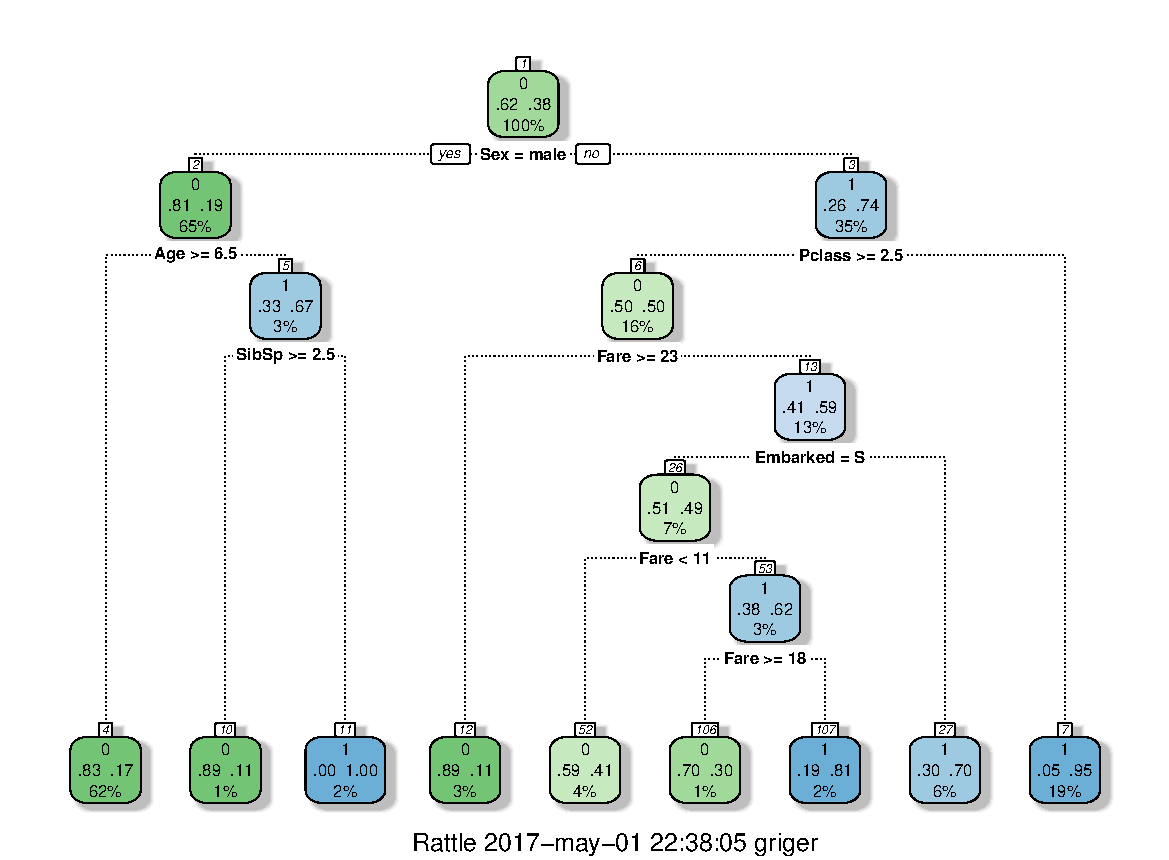
\includegraphics[width=\textwidth]{imgs/tree.pdf}
  \caption{Árbol de decisión}
\end{figure}

\begin{itemize}
\item En el primer nivel tenemos un nodo que predice que todos los pasajeros del conjunto de entrenamiento perecieron.
\item En el segundo nivel separamos los nodos según el sexo y tendríamos el modelo sexista del que hablamos anteriormente, sólo las mujeres se etiquetarán como sobrevivientes.
\item En la primera rama del nivel anterior tenemos el 65\% de la población. Aquellos hombres con más de 6.5 años te etiquetan como no-sobreviente, mientras que si el pasajero era un niño menor de 6.5 años (el 3\% de la población) entonces en caso de viajar con 3 hermanos o más, éste se supone sobreviviente.
\item Vemos también cómo aquellas mujers de tercera clase, el 19\% de la población, se supone que sobrevivieron al accidente.
\item Por otro lado aquellas de mejor clase que pagaron más de 23\$ el modelo supone que perecieron.
\end{itemize}

Por otro lado veamos la gráfica que podemos ver cuándo entrenamos un Random Forest del paquete \code{randomForest} en el tutorial de Megan Risdal: 

\begin{figure}[H]
  \centering
  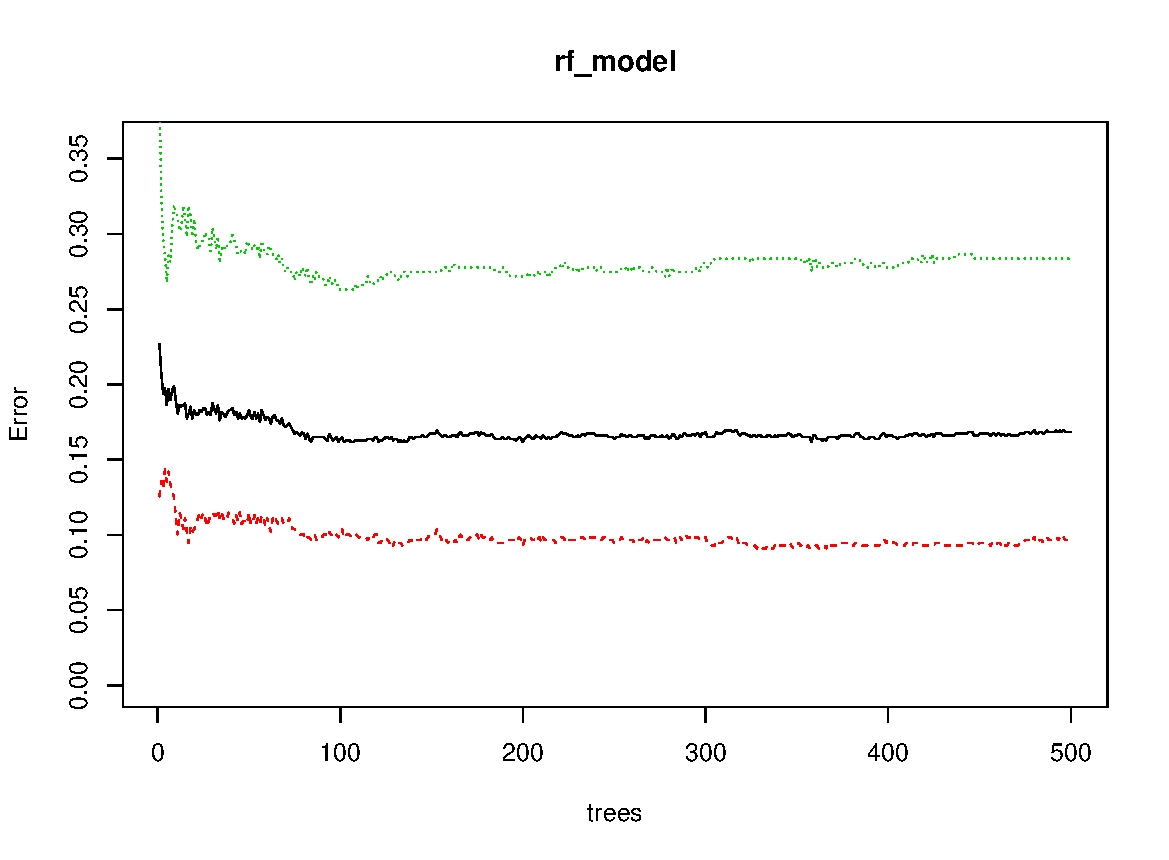
\includegraphics[width=\textwidth]{imgs/rf.pdf}
  \caption{Gráfica de un modelo de Random Forest}
\end{figure}

En la gráfica anterior se puede apreciar como varía la tasa de error, sobre el conjunto de entrenamiento, tanto para la clase mayoritaria como la minoritaria (también la total, la gráfica negra) según aumenta el número de árboles empleados en la clasificación. Como podemos ver, a partir de unos 70 árboles el error ya se estabiliza, con lo que, para el conjunto de train podríamos tener un modelo más simple para obtener una tasa de erro parecida. También es posible ver qué variables han tenido más importancia en la creación de los árboles según el índice de Gini:

\begin{figure}[H]
  \centering
  \includegraphics[width=\textwidth]{imgs/importance.pdf}
  \caption{Gráfica de un modelo de Random Forest}
\end{figure}

Como podemos ver el título del pasajero, su sexo y la tarifa que pagó son las más importantes, algo que esperábamos. Se puede ver cómo los atributos \code{Mother} y \code{Child} no son apenas relevantes, con lo que haberlas descartado en el proceso de clasificación ha sido una buena decisión, no sólo por la mejora en el resultado. Pasemos ya a analizar los resultados obtenidos por las distintas soluciones que hemos construido, comparando las distintas técnicas empleadas.\\

Como podemos ver los tres algoritmos (sin haber balanceado las clases ni limpiado ruido) empleados se comportan de forma muy parecida en el conjunto de train, en cambio a la hora de generalizar son los dos ensambles los que mejor funcionan, algo que era de esperar por la propia naturaleza de los algoritmos. Cabe señalar que xgboost, uno de los algoritmos que actualmente se consideran más potentes, obtiene el mismo resultado que Random Forest. Además para poder llegar a este resultado tuvimos que ajustar los parámetros de un modo adecuado de modo que no pecásemos de sobreajuste ni tampoco generásemos un modelo demasiado simple. Así se redujo el número de iteraciones que da el algoritmo (a 50, ya que con 30 la calidad de la solución diminuía), también se bajó el parámetro \code{eta} para que el modelo fuese menos conservativo en cuanto a lo que aprende en cada iteración y además ponemos el parámetro \code{subsample} a 0.5 de modo que en cada iteración sólo se emplee la mitad del conjunto de train en la construcción de los árboles para prevenir el sobreajuste.\\

El ensamble con esquema de votación del que hemos hablado anteriormente como podemos ver se comporta pero que el xgboost o el Random Forest por separado, como los modelos que obtuvimos a continuación fueron peores que estos primeros obtamos por no realizar ningún ensamble más con los nuevos modelos obtenidos tras las etapas de balanceo y de limpieza. Quizás si combinásemos todos los modelos podríamos obtener un mejor consenso, sería interesante probar esto como trabajo futuro.\\

Como podemos ver el balanceo de clases no mejor el resultado para ninguno de los algoritmos, sea cual sea la técnica empleada. Aunque la diferencia es mínima vemos cómo los algoritmos se comportan, en el test, mejor con el undersampling que con el oversampling, esto puede deberse a que estemos replicando datos y aumentando este ruido de clase, o quizás simplemente al replicar instancias del conjunto de entrenamiento lo que estemos haciendo es acusar aún más el problema del sobreajuste. SMOTE es la técnica de balanceo que, sin mejorar la mejor solución obtenida, hace que los algoritmo se comporten mejor (comparándolo con las otras técnicas de balanceo), quizás esto se deba a que estamos generando nuevos ejemplos y aunque estemos aumentando el ruido de clase no estamos provocando un mayor sobreajuste como sí que parece suceder con el oversampling.\\

Por último vemos cómo la combinación de SMOTE e IPF resulta muy mala para nuestro problema, estamos provocando, como se ve con el dato de la tasa de error en train, un sobreajuste muy elevado y esto si pensamos en que tenemos un problema con una separación entre las clases muy difusa resulta fatal. Realmente no tengo muy claro por qué se da esto y es algo que quiero analizar en un futuro. Parece que el hecho de balancear las clase y luego limpiar el ruido de la frontera lo único que hace es generar una división entre las dos clases muy marcada, algo que no se ajusta a la realidad del conjunto de entrenamiento, quizás ajustando los parámetros de balanceo y de limpieza de ruido pudiésemos obtener un mejor resultado.

\section{Conclusiones y trabajo futuro}

Como conclusiones destacaría en primer lugar lo complicado que puede resultar obtener un buen resultado en este problema y que por tanto aún queda mucho que aprender acerca de el análisis de datos para poder afrontar los problemas con mayor éxito. Además, señalar que en un conjunto de test tan pequeño es claro que pequeñas variaciones en las soluciones obtenidas provocan diferencias significativas de cara a la clasificación.\\

Además la metodología seguida por mí en este trabajo no ha sido del todo adecuada ya que por cuestiones de tiempo se dejó el cálculo de la tasa de acierto en train para el final del trabajo, y realmente el error de validación cruzada es algo muy importante que nos hubiese ayudado a detectar problemas de sobreajuste e intentar resolverlos.\\

Como aspectos positivos destacaría el aprendizaje, a través de este problema, de técnicas de balanceo de clases y de limpieza de ruido que hasta el momento no se habían tratado. Además en este problema destaca la importancia de la ingeniería de características para obtener buenos resultados y cómo se pone de manifiesto el teorema de No Free Lunch ya que un algoritmo tan potente como xgboost no ha sido capa de dar la mejor solución, quizás por los parámetros escogidos.\\

Algo que me gustaría haber probado, pero que por cuestiones de tiempo no se ha podido hacer, sería probar algoritmos de selección de características que, como vimos en clase, obtenían muy buenos resultados en la competición. También podría explorarse la opción de emplear redes neuronales, una técnica que está creciendo en importancia en los problemas de clasificación.\\

Sobre el trabajo que se ha realizado quizás sería interesante realizar un ajuste de parámetros más extenso, en particular, haciendo uso de las funcionalidades que nos ofrece \code{caret}, ajutar los parámetros para xgboost. Por último, aunque lo hemos descartado, sería interesante analizar el impacto del uso de una variable que recoja la cubierta en la que se alojó el pasajero. 

\begin{landscape}
\section{Listado de soluciones}
\pagestyle{empty}
\begin{table}[H]
\centering
\caption{Listado de resultados}
\label{my-label}
\begin{tabular}{|c|l|c|c|c|c|}
\hline
\rowcolor[HTML]{C0C0C0} 
Nº                                & \multicolumn{1}{c|}{\cellcolor[HTML]{C0C0C0}\textbf{Descripción preprocesamiento}}                                                                                                                                                                                         & \textbf{Alg. y soft. empleados}        & \textbf{\begin{tabular}[c]{@{}c@{}}Acierto\\ train\end{tabular}} & \textbf{\begin{tabular}[c]{@{}c@{}}Acierto\\ test\end{tabular}} & \textbf{Ranking} \\ \hline
\textbf{1}                        & \begin{tabular}[c]{@{}l@{}}El preprocesamiento de Megan Risdal:\\ - Extracción del título.\\ - Tamaño de famila e id de la misma.\\ - Imputación de valores perdidos, algunos con mice.\\ - Variables indicando si el pasajero es mayor de edad y si es madre.\end{tabular} & Random Forest del paquete randomForest & 0.8349884                                                        & 0.80383                                                         & 1034             \\ \hline
\rowcolor[HTML]{9AFF99} 
\textbf{2}                        & \begin{tabular}[c]{@{}l@{}}El preprocesamiento de Trevor Stephens:\\ - Variable indicando si es un adulto o no.\\ - Título del pasajero.\\ - Tamaño de la famila e id de la misma.\\ - Imputación de valores perdidos, árbol de decisión para la edad.\end{tabular}         & Random Forest del paquete party        & 0.8316678                                                        & 0.81340                                                         & 429              \\ \hline
\textbf{3}                        & El mismo de el tutorial de Stephens.                                                                                                                                                                                                                                        & rpart                                  & 0.8305505                                                        & 0.79426                                                         & 1469             \\ \hline
\textbf{4}                        & El mismo de el tutorial de Stephens.                                                                                                                                                                                                                                        & xgboost del paquete xgboost            & 0.8372921                                                        & 0.81340                                                         & 421              \\ \hline
\textbf{5}                        & El mismo de el tutorial de Stephens.                                                                                                                                                                                                                                        & Ensamble de rpart + xgboost + cforest  &                                                                  & 0.80861                                                         & 537              \\ \hline
\textbf{6}                        & El mismo de el tutorial de Stephen + down sampling.                                                                                                                                                                                                                         & cforest                                & 0.820283                                                         & 0.79426                                                         & 1691             \\ \hline
\textbf{7}                        & El mismo de el tutorial de Stephen + down sampling.                                                                                                                                                                                                                         & rpart                                  & 0.8202832                                                        & 0.78947                                                         & 2096             \\ \hline
\textbf{8}                        & El mismo de el tutorial de Stephen + down sampling.                                                                                                                                                                                                                         & xgboost                                & 0.8202832                                                        & 0.77990                                                         & 3186             \\ \hline
\textbf{9}                        & El mismo de el tutorial de Stephen + up sampling.                                                                                                                                                                                                                           & cforest                                & 0.8123288                                                        & 0.78469                                                         & 2720             \\ \hline
\textbf{10}                       & El mismo de el tutorial de Stephen + up sampling.                                                                                                                                                                                                                           & rpart                                  & 0.8132586                                                        & 0.73684                                                         & 6204             \\ \hline
\textbf{11}                       & El mismo de el tutorial de Stephen + up sampling.                                                                                                                                                                                                                           & xgboost                                & 0.8250809                                                        & 0.76555                                                         & 5044             \\ \hline
\multicolumn{1}{|l|}{\textbf{12}} & El mismo de el tutorial de Stephen + SMOTE.                                                                                                                                                                                                                                 & cforest                                & 0.9132704                                                        & 0.80383                                                         & 1007             \\ \hline
\multicolumn{1}{|l|}{\textbf{13}} & El mismo de el tutorial de Stephen + SMOTE.                                                                                                                                                                                                                                 & rpart                                  & 0.8923114                                                        & 0.77512                                                         & 3606             \\ \hline
\multicolumn{1}{|l|}{\textbf{14}} & El mismo de el tutorial de Stephen + SMOTE.                                                                                                                                                                                                                                 & xgboost                                & 0.9108267                                                        & 0.79426                                                         & 1722             \\ \hline
\multicolumn{1}{|l|}{\textbf{15}} & El mismo de el tutorial de Stephen + SMOTE + IPF.                                                                                                                                                                                                                           & cforest                                & 0.9994536                                                        & 0.77512                                                         & 3606             \\ \hline
\multicolumn{1}{|l|}{\textbf{16}} & El mismo de el tutorial de Stephen + SMOTE + IPF.                                                                                                                                                                                                                           & rpart                                  & 0.9983636                                                        & 0.77033                                                         & 4178             \\ \hline
\multicolumn{1}{|l|}{\textbf{17}} & El mismo de el tutorial de Stephen + SMOTE + IPF.                                                                                                                                                                                                                           & xgboost                                & 0.9978187                                                        & 0.77033                                                         & 4178             \\ \hline
\end{tabular}
\end{table}
\end{landscape}

\section{Material consultado}

\begin{itemize}
\item \href{https://www.kaggle.com/mrisdal/titanic/exploring-survival-on-the-titanic}{Tutorial de Megan Risdal}
\item \href{http://trevorstephens.com/kaggle-titanic-tutorial/getting-started-with-r/}{Tutorial Trevor Stephens}
\item \href{http://rpubs.com/Vincent/Titanic}{Tutorial que hace uso de un ensamble de varios algoritmos}
\item \href{https://triangleinequality.wordpress.com/2013/09/08/basic-feature-engineering-with-the-titanic-data/}{Tutorial sobre ingeniería de características}
\item Artículo \textbf{SMOTE–IPF: Addressing the noisy and borderline examples problem in imbalanced classification by a re-sampling method with filtering} de Francisco Herrera.
\item \href{https://github.com/dmlc/xgboost/blob/master/doc/parameter.md}{Sobre los parámetros de xgboost.}

\end{itemize}

\end{document}